% \documentclass[11pt,twoside,final]{ahudson-harvard}
% \usepackage{bm,float}
% \usepackage{times}
% \usepackage{url}
% \usepackage{graphicx}
% \usepackage{subfigure}
% \usepackage{verbatim}
% \usepackage{pgf}
% \usepackage{mathptmx}
% \usepackage{latexsym}
% \usepackage{url}
% \usepackage{LI}
% \usepackage{natbib}
% %\usepackage{parsetree}
% \usepackage{xspace}
% 
% \newcommand{\gis}{\textsc{gis}\xspace}
% \newcommand{\iis}{\textsc{iis}\xspace}
% \newcommand{\pos}{\textsc{pos}\xspace}
% \newcommand{\wsj}{\textsc{wsj}\xspace}
% \newcommand{\ccg}{\textsc{ccg}\xspace}
% \newcommand{\tag}{\textsc{tag}\xspace}
% \newcommand{\ltag}{\textsc{ltag}\xspace}
% \newcommand{\hpsg}{\textsc{hpsg}\xspace}
% \newcommand{\lbfgs}{\textsc{l-bfgs}\xspace}
% \newcommand{\bfgs}{\textsc{bfgs}\xspace}
% \newcommand{\cfg}{\textsc{cfg}\xspace}
% \newcommand{\pcfg}{\textsc{pcfg}\xspace}
% \newcommand{\nlp}{\textsc{nlp}\xspace}
% \newcommand{\dop}{\textsc{dop}\xspace}
% \newcommand{\lfg}{\textsc{lfg}\xspace}
% \newcommand{\pp}{\textsc{pp}\xspace}
% \newcommand{\cky}{\textsc{cky}\xspace}
% \newcommand{\gb}{\textsc{gb}\xspace}
% \newcommand{\mb}{\textsc{mb}\xspace}
% \newcommand{\ram}{\textsc{ram}\xspace}
% \newcommand{\mpi}{\textsc{mpi}\xspace}
% \newcommand{\cpu}{\textsc{cpu}\xspace}
% \newcommand{\parseval}{\textsc{parseval}}
% \newcommand{\trec}{\textsc{trec}\xspace}
% \newcommand{\epsrc}{\textsc{epsrc}\xspace}
% \newcommand{\dt}{\textsc{dt}\xspace}
% \newcommand{\hmm}{\textsc{hmm}\xspace}
% \newcommand{\ghz}{\textsc{ghz}\xspace}
% \newcommand{\rasp}{\textsc{rasp}\xspace}
% \newcommand{\ldc}{\textsc{ldc}\xspace}
% \newcommand{\gr}{\textsc{gr}\xspace}
% \newcommand{\qa}{\textsc{qa}\xspace} 
% \newcommand{\jj}{\textsc{jj}\xspace}
% \newcommand{\vbn}{\textsc{vbn}\xspace}
% \newcommand{\cd}{\textsc{cd}\xspace}
% \newcommand{\rp}{\textsc{rp}\xspace}
% \newcommand{\cc}{\textsc{cc}\xspace}
% \newcommand{\susanne}{\textsc{susanne}\xspace}
% \newcommand{\bandc}{\textsc{b{\small \&}c}\xspace}
% \newcommand{\ccgbank}{CCGbank\xspace}
% \newcommand{\candc}{\textsc{C}\&\textsc{C}\xspace}
% \newcommand{\cg}{\textsc{cg}\xspace}
% \newcommand{\penn}{\textsc{ptb}\xspace}
% 
% \newcommand{\develtwo}{\textsc{devel-2}}
% 
% \newcommand{\deps}{\mbox{\em deps}}
% \newcommand{\cdeps}{\mbox{\em cdeps}}
% \newcommand{\dmax}{\mbox{\em dmax}}
% 
% % commands for xyling
% \newcommand{\unode}[2][]{\K{#1$_{#2}$}}
% \newcommand{\bnode}[2][]{\K{#1$_{#2}$}\V}
% \newcommand{\vpmod}{}
% \newcommand{\bks}{$\backslash$}
% 
% \newcommand{\unify}{\equiv}
% \newcommand{\nounify}{\neq}
% \newcommand{\dest}{\textsc{dest}\xspace}
% 
% \newcommand{\nounary}{\textsc{nounary}\xspace}
% \newcommand{\cn}{\emph{\[citation needed\]}\xspace}
% 
% 
% \newcommand{\term}[1]{\emph{#1}}
% %\newcommand{\comment}[1]{\quote{#1}}
% 
% 
% 
% \begin{document}

\chapter{Analysing the Output of the \candc Parser}
\label{chapter:analysis}

\section{Introduction}

Much of the research in natural language processing is task oriented. The goal is to build a system that performs some useful work more quickly or accurately. Ideally, development of a solution to the problem proceeds in parallel, and the community progressively converges on the ideas that have proven effective.

Empirical evaluation is central to the success of this strategy. Systems are judged according to how closely their output corresponds to a sample of hand labelled data. Ultimately, we would like to be able to measure the contribution of each innovation according to its impact on the bottom line. Unfortunately, the reality is often more complicated.

For statistical parsers, `the bottom line' is itself very difficult to measure. Grammatical analyses are complex objects that are not easy to decompose, making it difficult to assign an accuracy for a partially correct response to a sentence. Grammatical theory is also an active area of research, so different parsers are often informed by different ideas of what the answer should be than the hand labelled data.

The other issue is that most statistical parsers --- like many other \nlp systems --- involve many interdependent design decisions. This makes it is very difficult to isolate and evaluate discrete contributions. The problem is compounded by the fact that the evaluation is problematic, since it makes it difficult to draw conclusions about how the system's behaviour changes when some detail is altered.

\subsection{Parser Evaluation}

Parser evaluation schemes usually give equal weighting to each attachment decision in a parse tree. But in English, most dependencies are quite local \cn, making most attachment decisions quite easy. This means that even a simple parser can score quite well, and forces systems into a narrow band of accuracy that does not necessarily reflect their performance.



%\comment{1 Find the average dependency distance paper}

%In order to learn how to improve statistical parsers, it helps to perform more detailed error analysis, sorting errors into linguistic categories**. CCG offers a good opportunity to do this, because of how informative its supertags are. We can look at a confusion matrix of supertags, and get an idea of what kind of misclassifications the parser is making.

\subsubsection{Bracket Accuracy}

The \parseval evaluation \citep{black91} measures the bracket precision and bracket recall, where a bracket is defined as a $(start word, label, end word)$ triple. This produces more fine grained results than measuring the accuracy of an entire sentence, since a single parse contains many brackets.

\citep{carroll02} summarised several problems with this, established in the literature over the many years in which the \parseval measures have been the main way English parsers have been evaluated. Perhaps the most prominent criticism has been that the evaluation is generally used to compare a parser's output against the Penn Treebank, linking development in the field to a single problematic annotation scheme \citep{beyond_parseval}.

More generally, several people have noted that a bracket does not correspond to a single linguistic decision (e.g. \citep{lin96}). Figure \ref{pp_attach} shows how a single attachment error can produce several incorrect brackets. When the PP node is incorrectly attached to the noun phrase deep in the parse tree, the boundary of every bracket above the NP changes.

\subsubsection{\ccg Dependency Accuracy}

Although the trees in Figure \ref{pp_attach} produce many different brackets, they differ on only one dependency. Dependencies correspond more closely to linguistic decisions, since each dependency represents exactly one attachment. However, treebank parsers do not necessarily recover dependencies intrinsically; and even if they do, the dependencies they recover may not match the dependencies in the evaluation set \cn.

A mapping from a constituency parse to a dependency representation may also involve some loss of information \citep{atwell96}. In practice this is seldom a concern, because attention has been focused on skeletal, or shallow, parsing that does not recover the trace nodes which represent the information that would be lost.

\subsubsection{Grammatical Relations}

One of the problems for parser evaluation is that grammar development is an unsolved problem. This means that most formalisms that are useful for parsing also have trouble representing all of the information it would be useful to recover. \citet{briscoe02} therefore proposed an evaluation format that is not linked to a parsing formalism. They propose a dependency-based format that relaxes some of the assumptions that make dependency parsing tractable, making the format far more flexible. The scheme is a set of binary and ternary grammatical relations loosely based on Lexical Functional Grammar F-structures, forming a dependency graph.

The most important advantage of the \citeauthor{briscoe98} grammatical relations over previous evaluations is that it rewards systems that produce more informative output, correcting a significant weakness of the \parseval measures. Skeletal parses based on the Penn Treebank leave a lot of important grammatical information unrecovered: complements and adjuncts are not distinguished, long range dependencies are not recovered, noun phrases are not bracketed, and many constructions are treated inadequately. By stepping back from the problem of grammar development and focusing on a representationally adequate format, the grammatical relations evaluation is able to offer a more complete assessment of how useful a parser will be for information extraction.

The principle downside of the grammatical relations evaluation is that parsers are unlikely to recover dependencies in this format directly. Instead, some mapping must be used from the parser's native output into the evaluation format. This mapping is potentially labour intensive, and is almost certain to be lossy --- leading to some amount of noise in the evaluation.

\subsection{Evaluation and Parser Development}

The grammatical relations evaluation is designed to be as robust as possible to differences in the grammars underpinning two different parsers. But there is another use case for evaluation measures where this is not a requirement. The development of a statistical parser involves dozens of decisions whose impact it would be useful to examine empirically. In this case, the two parsers being compared are almost identical. This calls for an evaluation that is maximally \emph{sensitive}, rather than one that is maximally \emph{robust}.

\section{Contributions}

In this chapter, we undertake a detailed examination of the performance of the \candc parser. The examination is specifically tuned to the parser's design: we want to isolate each processing stage and parameter, and consider its impact on the parser's output. This yields several research contributions.

Firstly, we carefully examine details of the \candc parser that have not received much attention in publications about the system to date. As \citet{bikel} argued in his examination of the details of the Collins parser \citet{collins}, the details of complicated systems are often critical to reproducing results. Our second contribution is a demonstration of this point, by examining the impact of these details on the parser's performance.

Perhaps the most important contribution of this work is its service as an example of how to thoroughly analyse a complicated NLP system. We show how isolating each processing stage requires a different set of descriptive statistics. Once the processing stage has been isolated, it is much easier to systematically explore different parameter settings, providing a more principled way to select appropriate values.

\subsection{Relevance to Thesis}

This thesis presents an extension to \ccg that we argue addresses a long-standing problem in categorial grammars, allowing faster and more accurate \ccg parsing. In Chapter \ref{chapter:nounary}, we also introduce a \ccg corpus that does not use any rules not licensed by \ccg. The analysis presented in this chapter allows us to compare these two corpora to \ccgbank in detail, and show how their grammars and lexicons differ. This allows us to evaluate the hypothesis presented in Chapter \ref{chapter:cat_deps} much more accurately, as we describe when we implement the solution proposed in Chapter \ref{chapter:hat_cats} in Chapter \ref{chapter:hat_corpus}.


\section{Overview of the Parsing Pipeline}

The \candc parser consists of a tightly integrated supertagger and parser that operate after a part of speech tagger, as described in Section \ref{sec:background:parser}. In order to study how to improve the system, we need a way to discover where errors are introduced as a sentence travels through the parsing process. We identify five stages of interest in which an error can occur:

\subsection{Part of Speech Tagging}

If a word has been assigned an incorrect part of speech (POS) tag, it is highly likely to disrupt the rest of the analysis, since it is almost certain to be assigned an incorrect \ccg category. It is therefore useful to isolate POS tagging errors and consider them separately. For this reason most parsing systems report results using gold standard POS tags, in addition to results when automatic POS tags were used. For our purposes, gold standard POS tags are more useful, since we are not interested in tuning the POS tagger, only the parsing system. We do not discuss results using automatically calculated POS tags in this section.

\subsection{Category Lexicon}

The \candc supertagger infers a \term{tag dictionary} from the training portion of \ccgbank. This tag dictionary is used to filter the model's tag decision in the following way:

%\comment{TODO: freq cutoffs etc here.}

Even a perfect model, then, would not be able to offer perfect category assignments to the parser: in some number of cases, the correct tag is unavailable. To investigate why and how often this occurs, we would like to know:

\begin{enumerate}
 \item How often the correct category has never occurred in the training data
 \item How often the correct category occurs between 1 and $\theta$ (the frequency threshold at which categories are discarded from the category set)
 \item How often the correct category is in the category set, but has never occurred for the given word
 \item How often the correct category has been seen with the given word between 1 and $\theta'$ (the frequency threshold at which categories are discarded from a word's tag dictionary)
\end{enumerate}

The category filtering decisions are \emph{ad hoc} engineering solutions to sparse data problems in the \ccgbank training data. By analysing this stage of the parsing process, we hope to find informed ways of setting these parameters. This will help adjust the parser for different training data, such as a corpus for a different language or different \ccg analyses. It might also produce better values for the current English \ccgbank.

\subsection{Supertag Model}

The \candc supertagger uses a maximum entropy based sequence tagger, following \citet{ratnaparkhi}. The tagger uses a variable width beam to offer a set of categories for each word to the parser. If no analysis can be found for the analysis offered, the beam is increased and the parser tries again with the expanded set. This process continues until the parser can return an analysis, or it has failed after the supertagger has supplied an analysis with its maximum beam width. Section \ref{background:stagger} describes details of the supertagger's sequence tagging model. Section \ref{background:integration} describes the integration of the parser and supertagger in more detail.

The following questions will help us guage the effectiveness of the supertagger's model:

\begin{enumerate}
 \item How often is the correct supertag present in the beam at each width offered to the parser?
 \item How large is the category set the tagger offers at each beam width?
 \item How often does the supertagger's analysis contain the correct tag for each word at each beam width?
 \item How much of the probability mass does the model assign to the correct tag?
\end{enumerate}

\subsection{\ccg Parser}

The \candc parser uses a packed chart to generate all analyses it can produce with a given set of categories from the supertagger. The parser implements all \ccg combinators that occur in \ccgbank:

\begin{itemize}
 \item Forward application
 \item Backward application
 \item Forward composition
 \item Backward composition
 \item Backward crossing composition
 \item Conjunction
\end{itemize}

In addition, it implements several of the unary and binary non-combinatory production rules found in \ccgbank. These include punctuation rules, but also the type-changing rules described in Section \ref{background:ccgbank}. However, these production rules have a heavy-tailed distribution, so the parser does not implement all of them. Type-raising is implemented in much the same way as the non-combinatory unary rules --- as a set of specific unary productions that can be invoked during parsing.

We can describe the rate at which the parser finds at least one correct analysis as its \emph{recall}. We can also assume that the total number of analyses it finds is inversely related to its \emph{precision}: the proportion of correct to incorrect analyses it produces. This assumption is not necessarily true, since multiple \ccg derivations may yield the correct dependencies for a sentence. However, when the parser produces hundreds of thousands of analyses --- as is often the case for long sentences --- the vast majority of them ar probably incorrect.

The following questions will help us understand more about the recall and precision of the parser, and the relationship between the two:

\begin{enumerate}
 \item How often does the parser fail to find a correct analysis with the correct categories?
 \item How often is the failure due to composition constraints that cause it to fail to produce a valid composition production?
 \item How often is the failure due to a type-raise category that could not be found?
 \item How often is it due to a missing non-combinatory rule?
 \item How do chart sizes grow with respect to sentence length?
 \item What other features of a sentence predict chart size?
 \item What are the effects of grammaticalised type-raising on chart sizes?
 \item What are the effects of the non-combinatory rules on chart sizes?
\end{enumerate}

\subsection{Parser Model}

The \candc parser uses maximum entropy modelling to train a discriminative classifier on a feature forest generated from a packed chart. Typically, the model will have to select an analysis from hundreds of thousands of possibilities, as the chart will be seeded with multiple categories per word.

We raise the following questions about the parser model:

\begin{enumerate}
 \item Is better accuracy achieved by retaining ambiguity (in the form of a wider supertagging beam) and letting the model resolve it, or is it better to use a narrow beam to reduce the number of analyses?
 \item What kinds of phenomena does the model struggle to classify accurately, other things being equal?
\end{enumerate}
 
\section{Lexicon Analysis}

In this section, we analyse a category lexicon compiled from the \ccgbank training section, 02-21. We then investigate the coverage of this lexicon against section 00.

Our analysis is structured around two parameters that \candc use to control the size of the lexicon they extract from the training section of the corpus. First, categories that occur below a frequency threshold $F_c$ are ommited from the category set. \candc set $F_c$ to 20. We refer to this parameter as the \emph{category frequency threshold}

The other parameter we explore relates to the compilation of the \emph{tag dictionary}. The tag dictionary is the set of category that the supertagger is allowed to assign to a word. The most important parameter here is $F_w$: the number of times a word must occur in the training data before a tag dictionary is built for it. Words whose frequency falls below this threshold can receive any category in the tag dictionary of its POS tag --- a large set. We refer to this parameter as the \emph{tag dictionary activation threshold}.



\subsection{Category Frequency Thresholds}

Figure \ref{analysis:catfreq} plots the impact of the category frequency threshold on four statistics calculated on Section 00:

\begin{enumerate}
 \item The proportion of tokens whose category is in the category set
 \item The proportion of sentences that have no tokens with a category missing from the category set
 \item $H(w|c)/max(H(w|c)$, where $H$ is the average information required to assign a category to a token given its lemma, and $max(H(w|c))$ is the value observed for this measure when the category threshold is set to 0 (TODO: yeah I know that made no sense. Crap.)
 \item The proportion of categories with the category frequency threshold at $N$, compared to the number of categories with the category frequency threshold at 0.
 \end{enumerate}
 
\begin{figure}
\rotatebox{270}{\scalebox{0.45}{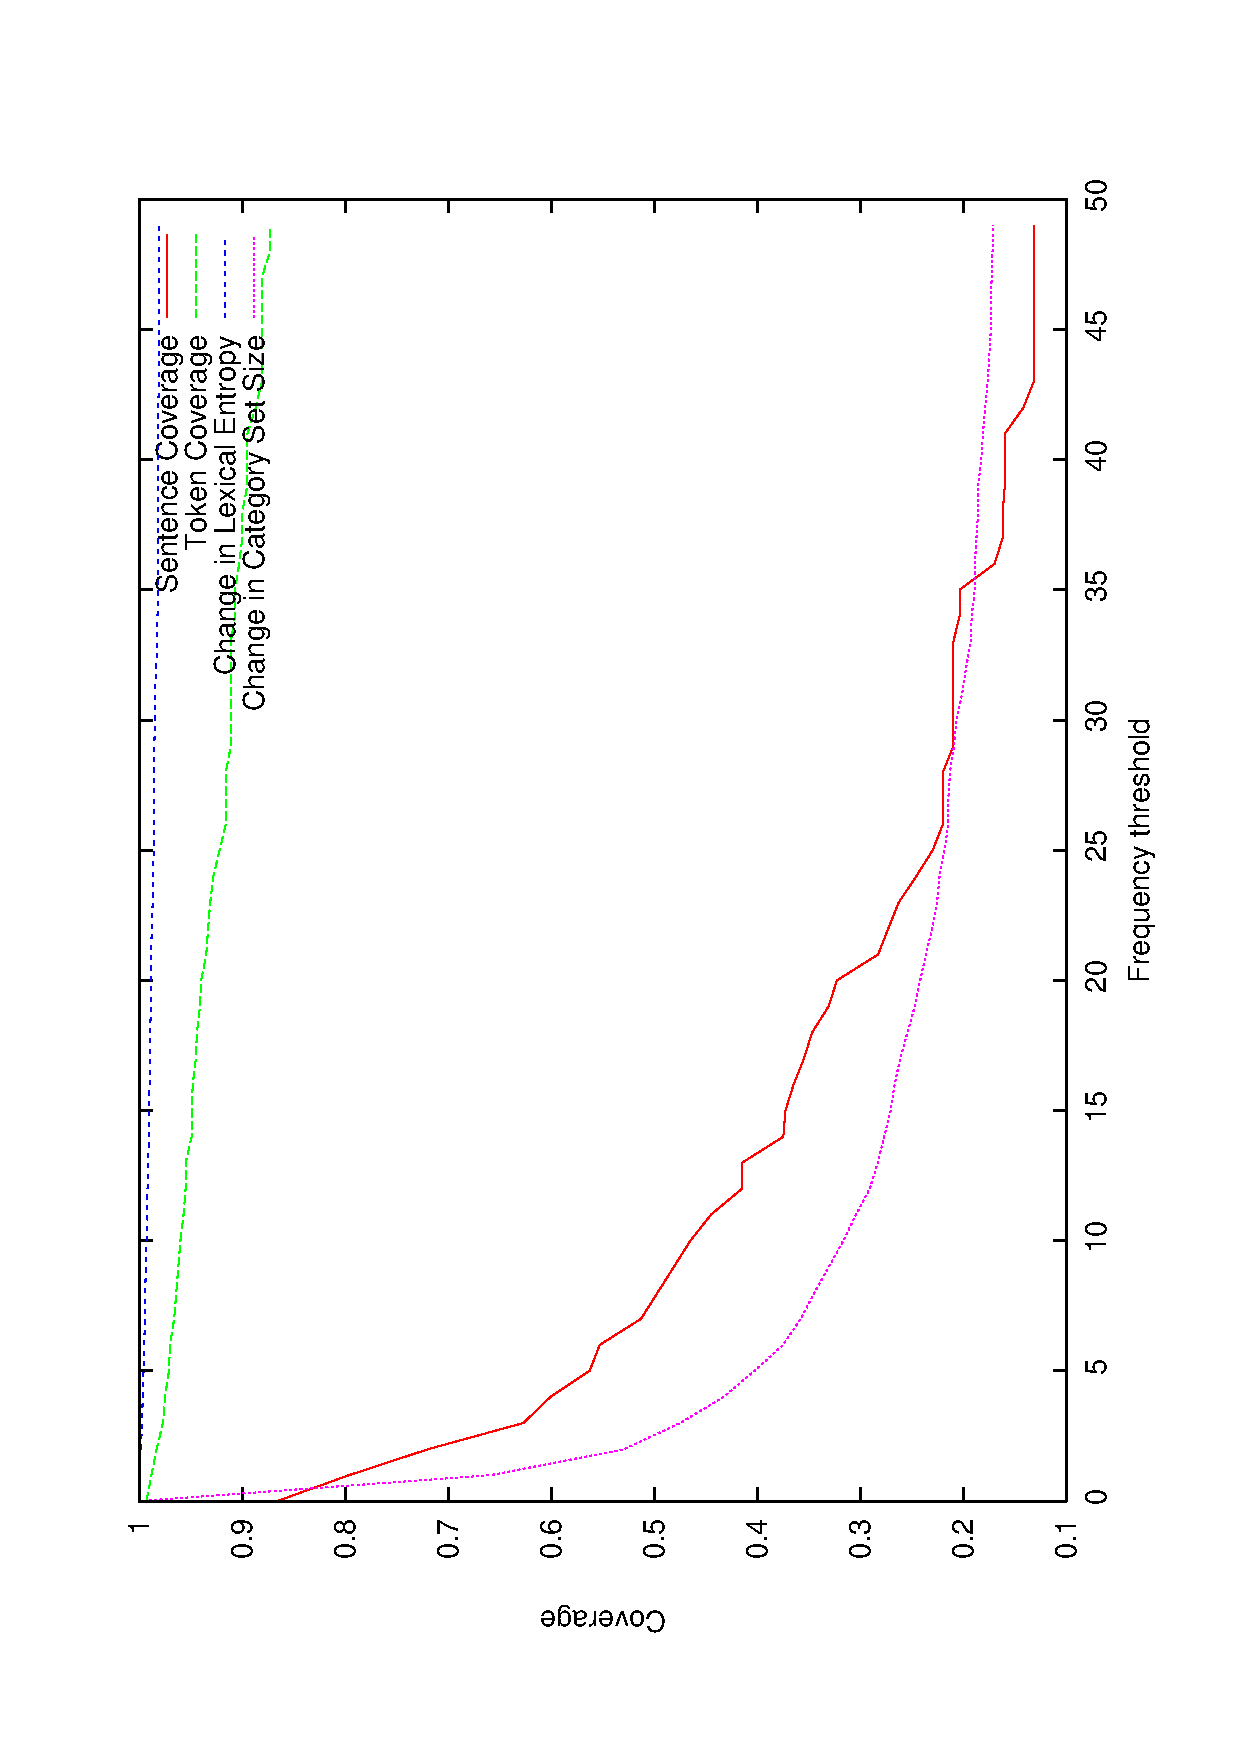
\includegraphics{./analysis/cover_entropy}}}
\label{analysis:catfreq}\caption{Change in various statistics as category frequency threshold is increased.}
\end{figure}

Figure \ref{analysis:catsize} shows the number of categories more frequent than the threshold $\theta_c$. This shows the heavy-tailed nature of the category set. Some of this is the result of noise introduced during the conversion process, either through errors in the Penn Treebank source text, or imperfections in the conversion heuristics. Other rare categories simply represent rare argument constructions or syntactic phenomena that do not occur often in the Wall Street Journal corpus, such as imperative mood verbs. Table \ref{analysis:cats} shows some example categories, a gloss of the syntactic construction they largely represent, and their frequency.

We are also interested in how these categories are distributed with respect to the words in the data. That is, how ambiguous, on average, is the category of a given word? We measure this as the conditional entropy of the category set $C$ given a particular word $w$:

\begin{eqnarray}
H(C|w)
\end{eqnarray}

One way to consider the average ambiguity would be to simply take the mean entropy conditioned on each word in the lexicon. However, we prefer to calculate the mean entropy of each token in the data, which amounts to weighting each word's ambiguity according to its frequency. Figure \ref{analysis:ambiguity} shows how the expected category ambiguity of each token in the corpus changes as we use a higher frequency threshold for inclusion in the words' tag dictionary.



%\comment{TODO: I suck at explaining maths, the above is horrible. Fix, and learn how to do this properly...}

Increasing the frequency thresholds reduces the number of sentences that can be parsed correctly, as two analyses with different lexical categories cannot yield identical dependencies. Figure \ref{analysis:coverage} shows how coverage over the training data and category ambiguity are related: higher tag dictionary frequency thresholds ($\theta_t$) result in lower category ambiguity, but also lower coverage.

\begin{table}
\begin{tabular}{l|l}
Meaning & Symbol\\
$\theta_{c}$ & Category set frequency threshold\\
$\theta_{t}$ & Tag dictionary frequency threshold\\
$\theta_{w}$ & Word frequency threshold for using a tag dictionary\\
$F_{c}$ & Frequency of a category in the training data\\
$F_{w}$ & Frequency of a word in the training data\\
$F_{wc}$ & Frequency of a $(word, category)$ pair in the training data\\
$\beta$ & Lower $\beta$ values increase the width of the supertagger's beam\\

\end{tabular}
\end{table}

\subsection{Tag Dictionary Activation Threshold}

Table \ref{analysis:ood} shows how often the various out of dictionary errors occur using the default \candc parameter settings, in \develtwo and section 00.

\begin{itemize}
\item $F_c=0$ shows how many sentences contained at least 1 category that occurred 0 times in the training data
\item $F_c>0<10$ shows how many sentences contained at least 1 category that occurred between 1 and 10 times in the training data, and was thus excluded from the category set.
\item $F_c>10<20$ shows how many sentences contained at least 1 category that occurred between 10 and 20 times in the training data, and was thus excluded from the category set.
\item $F_{wc}$ shows how many sentences contained at least 1 word that used a tag dictionary (as the word occurred more than 20 times), but the word never occurred with the required category.
\item $F_w>20 F_wc>0<10$ shows how many sentences contained at least 1 word that used a tag dictionary (as the word occurred more than 20 times), but the word occurred with the required category too infrequently to have it in its tag dictionary.
\end{itemize}
\begin{table}
\begin{tabular}{l|r|r}
 & 00 & Devel2\\ \hline
$F_c = 0$ & 0.009 & 0.008\\
$F_c <= 10$ & 0.04 & 0.047\\
$F_c <= 20$ & 0.062 & 0.075\\
$F_wc = 0$ & 0.117 & 0.133\\
$F_wc < 5$ & 0.328 & 0.352\\
\end{tabular}\caption{Proportion of sentences subject to various out of dictionary errors.}\label{analysis:ood}
\end{table}




The table shows that 32.8\% of sentences contain at least one word that uses a tag dictionary that does not include the correct category. These sentences are guaranteed to contain parse errors --- no matter what the supertagger and parser models do, a correct category analysis cannot be supplied, which means a correct parse cannot be built.

When compared to the number of tag dictionary errors, the number of infrequent category errors is quite low. Approximately 6\% of sentences contained a word whose category was too infrequent to be included in the category set.

One way to reduce the number of tag dictionary errors is to simply increase the frequency threshold at which a word uses a tag dictionary. Figure \ref{analysis:td_thresh} plots the proportion of tag dictionary error sentences at different thresholds, along with the percentage of tokens that invoke a tag dictionary.

The figure shows that the proportion of sentences with a tag dictionary error falls much faster than the proportion of tokens using a tag dictionary. This suggests that if we increase the threshold, we will be able to recover some of the out of dictionary errors while still getting the benefit of a tag dictionary for almost as many tagging decisions. 

\begin{figure}
\rotatebox{270}{\scalebox{0.45}{\includegraphics{./analysis/td_fails.eps}}}
\end{figure}


\section{Supertag Model Analysis}

Table \ref{analysis:stag_model} provides statistics about the supertagger's performance.

\begin{table}\centering
\begin{tabular}{l|r|r}
Measure & W/o tag dict & w/ tag dict\\
\hline
Mean gold prob & 0.897 & 0.93\\
Mean top prob & 0.93 & 0.946\\
Mean gold rank & 6.146 & 1.021\\
Mean required beta & 0.953 & 0.976\\
\end{tabular}\label{analysis:stag_model}\caption{How well does the supertagger assign its probability to the correct category?}
\end{table}

\begin{enumerate}
\item Mean probability assigned to correct category
\item Mean probability assigned to top category
\item Mean rank of correct category
\item Mean beta level required to recover correct category
\end{enumerate}

\begin{table}
\centering
\begin{tabular}{r|r|r|r|r|r}
Beta level & \% of tokens & Sent. completion rate & Mean ranks & Mean max $P$ & Mean gold $P$\\
\hline
1.0 & 0.955 & 0.360 & 1.000 & 0.962 & 0.962\\
0.9 & 0.003 & 0.375 & 1.646 & 0.457 & 0.435\\
0.8 & 0.003 & 0.392 & 1.669 & 0.478 & 0.407\\
0.7 & 0.004 & 0.414 & 1.737 & 0.490 & 0.368\\
0.6 & 0.005 & 0.436 & 1.663 & 0.529 & 0.342\\
0.5 & 0.004 & 0.457 & 1.619 & 0.554 & 0.303\\
0.4 & 0.004 & 0.485 & 1.486 & 0.602 & 0.270\\
0.3 & 0.005 & 0.518 & 1.513 & 0.643 & 0.223\\
0.2 & 0.007 & 0.567 & 1.348 & 0.687 & 0.170\\
0.1 & 0.010 & 0.649 & 1.138 & 0.749 & 0.109\\
\end{tabular}\caption{Supertagger statistics divided according to the beta level required to retrieve the correct category for each token.}
\end{table}

%\comment{TODO: Discussion of these results}

Table \ref{analysis:stag_beta} shows the supertagger's performance at various $\beta$ settings. A category whose assigned weight is within $c\beta$, where $c$ is the highest weight the model has assigned for that tagging decision, will be included in the set of categories the supertagger provides to the parser for that word.

Unfortunately, the fact that the parser has found a parse with the supertag analysis provided to it is no guarantee that the supertag analysis is correct. The parser may have built an incorrect parse out of incorrect categories. The parser may even fail to find a parse even if it is provided a perfect supertag analysis.

Instead of looking at whether the parser can return an analysis, we are interested in whether the sentence's analysis is \emph{complete}. We say that a sentence's analysis is complete if the supertagger supplies the correct category for every token. Note that the correct category need not be the only category returned. At $\beta < 1.0$, the supertagger may return multiple categories for the word, depending on the probability distribution it has assigned.

Tthe \textbf{Sent. completion rate} column of Table \ref{analysis:stag_beta} shows how the sentence completion rate increases as the $\beta$ parameter is relaxed, and more categories are added. The \textbf{\% of tokens} column shows how many tokens required this $\beta$ level to receive the correct category. For instance, if a token required $\beta=0.4$, then
\begin{eqnarray}
0.4 <= P(gold)*c <= 0.5
\end{eqnarray}

where $P(gold)$ is the probability the tagger assigned to the correct category, and $c$ is the maximum probability it assigned to a category for that word. The \textbf{Mean rank} column shows where the correct category fell in the distribution for tokens that required that $\beta$ level.



%we accept an analysis --- a sequence of category sets provided by the supertagger --- if every category set contains the correct tag for that word. If we do not accept the analysis, we increase the beam width by lowering the $\beta$ parameter and try again.

%This allows us to study the supertagger's performance at each $\beta$ level without any interaction with the parser. It also allows us to define which words are at fault for an analysis failure. At each $\beta$ level, we are only interested in reporting results for words where the correct category has only just been added to the category set. Otherwise, we will be including words with easy tagging decisions in the statistics for low $\beta$ values, simply because those words happen to occur in the same sentence as a word with a more difficult tagging decision. We include a final $\beta$ value, 0.0, to ensure that all words whose category can be assigned are included in the analysis.

\begin{enumerate}
\item Average category set size for words analysed correctly at $\beta$
\item Percentage of sentences analysed correctly at $\beta$
\item Average weight assigned to first weighted category at $\beta$
\item Percentage of tokens where correct category assigned highest weight at $\beta$
\item Average rank of correct category in category set
\item Average entropy of weights in category set
\end{enumerate}

\begin{figure}
\rotatebox{270}{\scalebox{0.45}{\includegraphics{./analysis/pass_rates.eps}}}
\end{figure}


%\comment{TODO: Discussion of these results}

\section{Parser and Grammar Analysis}

There are several ways the \candc implementation of the \ccgbank grammar can fail to generate the correct derivation, given a correct category analysis. Table \ref{analysis:grammar_recall} shows how often the various events occur:

\begin{enumerate}
 \item The percentage of sentences where parsing fails
 \item The percentage of failures caused by the composition constraints
 \item The percentage of failures caused by missing type raised categories
 \item The percentage of failures caused by a missing non-\ccg unary production
 \item The percentage of failures caused by a missing non-\ccg binary production
\end{enumerate}

%\comment{TODO: Discussion of these results}

Table \ref{analysis:grammar_recall} is essentially concerned with the parser's \emph{recall}. However, the \emph{precision} of the parser is also important. This is why the parser imposes composition constraints and does not support the long tail of infrequent non-\ccg production rules. Supporting additional rules means introducing more ambiguity into the grammar, which means far larger chart sizes.

Table \ref{analysis:grammar_precision} shows how support for various aspects of the \ccgbank grammar affect the parser's precision. Because chart sizes grow extra-linearly, we report the number of analyses in log space.

\begin{enumerate}
 \item Chart size and coverage with no composition rules
 \item Chart size and coverage with type raising lexicalised
\end{enumerate}

\section{Parser Model Analysis}

Once the chart has been created, a maximum entropy model is used to select the most likely parse. Section \ref{background:parser_features} describes the features \citet{candc} use

\begin{enumerate}
 \item Is better accuracy achieved by retaining ambiguity (in the form of a wider supertagging beam) and letting the model resolve it, or is it better to use a narrow beam to reduce the number of analyses?
 \item What kinds of phenomena does the model struggle to classify accurately, other things being equal?
\end{enumerate}




% \section{SuperTag Confusion}
% 
% Table \ref{stag:confused} shows the gold and test supertag pairs that account for the most supertag misclassifications made by the parser on section 00 of \ccgbank. The table refers to the tags selected by the parser. In Section \ref{dist-labour} we explore where in the parsing pipeline these errors are introduced. The table shows:
% 
% \begin{itemize}
% \item The frequency of the misclassification pair
% \item The proportion of misclassifications the pair constitutes
% \item The tag which the parser selected
% \item The correct tag from \ccgbank
% \item The frequency of the predicted tag
% \item The frequency of the gold tag
% \item The parser's accuracy at predicted the gold tag, measured by f-score
% \end{itemize}
% 
% \comment{I consistently get reviewer comments asking what some column in a table refers to, so I want to keep an eye on the issue and get better at describing my tables.}
% 
% \begin{table}
% \begin{tabular}{r|r|c|c}
% 175 & 4.9\% & \cf{NP\bs NP} & \cf{N}\\
% 158 & 4.5\% & \cf{N} & \cf{N/N}\\
% 151 & 4.3\% & \cf{((S\bs NP)\bs (S\bs NP))/NP} & \cf{(NP\bs NP)/NP}\\
% 118 & 3.4\% & \cf{PP/NP} & \cf{((S\bs NP)\bs (S\bs NP))/NP}\\
% 113 & 3.2\% & \cf{((S\bs NP)\bs (S\bs NP))/NP} & \cf{PP/NP}\\
% 108 & 3.0\% & \cf{(NP\bs NP)/NP} & \cf{((S\bs NP)\bs (S\bs NP))/NP}\\
% 95 & 2.7\% & \cf{N/N} & \cf{N}\\
% 74 & 2.1\% & \cf{PP/NP} & \cf{(NP\bs NP)/NP}\\
% 65 & 1.8\% & \cf{(NP\bs NP)/(NP\bs NP)} & \cf{N/N}\\
% 33 & 1.4\% & \cf{(N/N)/(N/N)} & \cf{N/N}\\
% 32 & 0.9\% & \cf{(NP\bs NP)/NP} & \cf{PP/NP}\\
% 27 & 0.8\% & \cf{((S[ng]\bs NP)/PP)/NP} & \cf{(S[ng]\bs NP)/NP}\\
% 27 & 0.8\% & \cf{(S\bs NP)\bs (S\bs NP)} & \cf{N}\\
% 24 & 0.7\% & \cf{((S[dcl]\bs NP)/PP)/NP} & \cf{(S[dcl]\bs NP)/NP}\\
% 21 & 0.6\% & \cf{N/N} & \cf{NP[nb]/N}\\
% 21 & 0.6\% & \cf{(S[dcl]\bs NP)/PP} & \cf{S[dcl]\bs NP}\\
% 20 & 0.6\% & \cf{NP[expl]} & \cf{NP}\\
% 20 & 0.6\% & \cf{S[adj]\bs NP} & \cf{N}\\
% 20 & 0.6\% & \cf{S[dcl]\bs NP} & \cf{S[dcl]\bs NP)/PP}
% \end{tabular}
% \end{table}
% 
% Unsurprisingly, infrequent tags are often misclassified as frequent tags they resemble. But looking a little more closely, we can see that almost all of these errors fall into three broad categories:
% 
% \begin{itemize}
% \item \np structure errors
% \item \pp attachment errors
% \item Complement/adjunct confusion errors
% \end{itemize}
% 
% Of these, \np structure and complement/adjunct confusions relate to two of the major known problems with \ccgbank, inherited from the annotation limitations in the Penn Treebank. \pp attachment is a major source of syntactic ambiguity in English, and a persistent area of difficulty for statistical parsers^4.
% 
% \comment{4. Citation needed}
% 
% In order to make these observations, we need to generalise over the \ccg categories. We need to be able to see which tags relate to \np structure, which tags represent adjuncts, and which tags are likely to represent prepositional phrases. If we could draw these generalisations systematically, we would be in a much better position to find interesting patterns.
% 
% We therefore draw up a heirarchy and sort tags into it. The nodes of the heirarchy are generic category forms. The generic forms we use are:
% \begin{itemize}
% \item \cf{X}: A portion of a category that must be matched exactly somewhere else. For instance, an adjunct is defined as a category of the form \cf{X/X} or \cf{X\bs X}.
% \item \cf{\vbar}: Either \cf{/} or \cf{\bs}
% \item \cf{\$}: Some set of arguments.
% \end{itemize}
% 
% 
% 
% 
% 
% \section{Out of Dictionary Errors}
% 
% \section{Investigating the Category Set}
% 
% \section{Lessons from Other Formalisms}
% 
% \section{Tentative Conclusions}
%\end{document}